

\documentclass[]{deedy-resume-openfont}


\begin{document}



%%%%%%%%%%%%%%%%%%%%%%%%%%%%%%%%%%%%%%
%
%     TITLE NAME
%
%%%%%%%%%%%%%%%%%%%%%%%%%%%%%%%%%%%%%%


\namesection{Joel Mateo}{Moreno Quintero}{ 

\centering
\href{mailto:joelmateo3@hotmail.com}{joelmateo3@hotmail.com} | 300-5605962 | 319-5662325\\
\urlstyle{same}\url{https://co.linkedin.com/in/mateo-moreno-612a45a2} \\
}

\vspace*{0.6cm}

\begin{minipage}[c]{.6\textwidth}
\section{Información Personal}
\vspace*{0.4cm}
\begin{flushleft}
	Ingeniero Electrónico\\
    Nacido en Bogotá el 25 Diciembre 1992\\
    Estado Civil: Soltero\\
    Cedula: 1022380344 \\
    Dirección: Diag 5 No 37 b - 60, Bloque 1 Apt 301\\
    Bogotá, Colombia
   
\end{flushleft}\normalsize
\end{minipage}
\hfill
\begin{minipage}[c]{.35\textwidth}
\begin{flushright}
\vspace*{0.4cm}
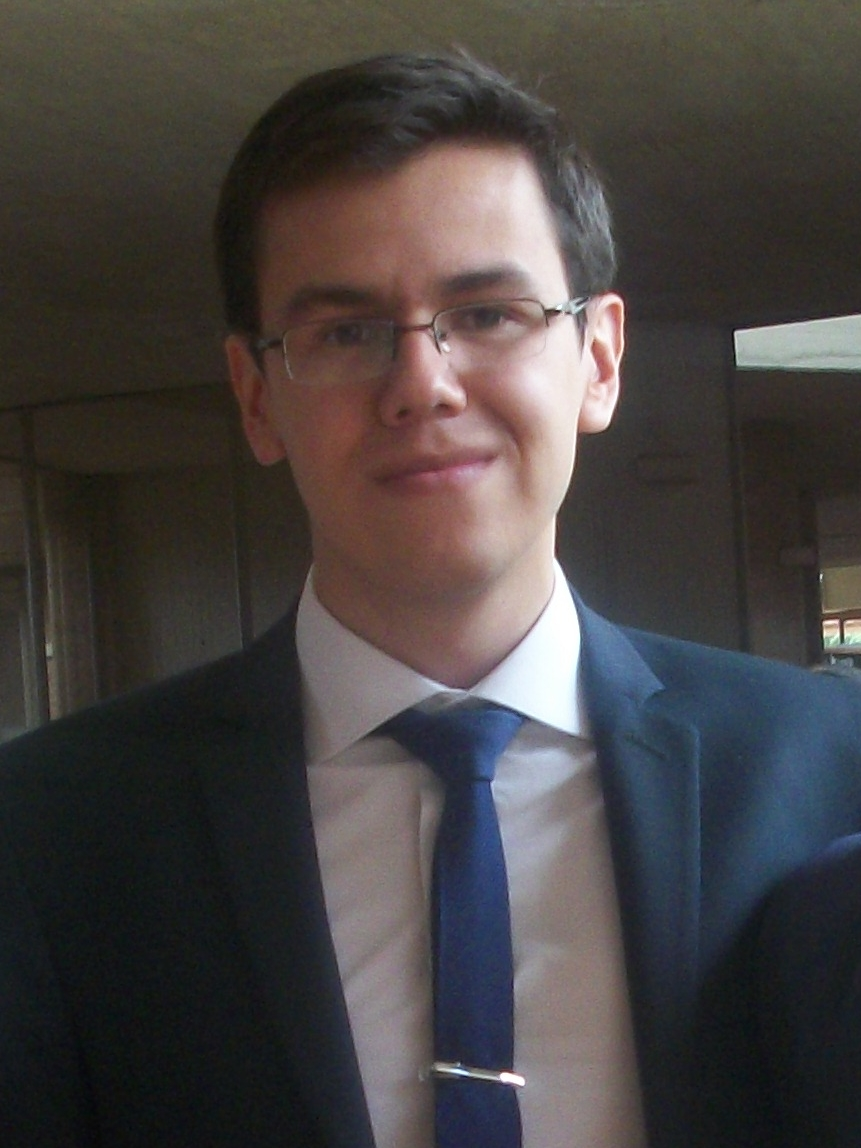
\includegraphics[width=80 pt]{100_9281.JPG}
\hspace*{0.6cm}
\end{flushright}

\end{minipage}
\vspace*{0.3cm}

\section{Perfil Profesional}
Ingeniero Electrónico de la Universidad Distrital  Francisco José de Caldas, comprometido y diligente en el trabajo, con habilidades para innovar o liderar proyectos,  con iniciativa para aportar soluciones  y aprender de nuevos desafíos presentados, con facilidad de trabajar en equipo. Tengo  experiencia en administración de TI, servicios integrados y software de IBM,  además de conocer cómo funciona una empresa reconocida internacionalmente como IBM.  Tengo predisposición para aprender y adoptar funciones en gestión y administración de proyectos o ventas preferiblemente enfocadas al sector de la tecnología. También  poseo habilidades para el diseño de sistemas electrónicos  inteligentes  y manejo de distintos lenguajes de programación, con un perfil académico enfocado hacia el control, la automatización y la inteligencia computacional.  

\sectionsep

%%\begin{center}
%%\huge\color{subheadings}\custombold{LIFELONG LEARNER}
%%\end{center}

\section{Experiencia}

\runsubsection{Informática Servicios y soluciones de Colombia S.A - Subsidiaria IBM}
\descript{|Administrador de la suite de productos IBM BigFix y Tivoli Monitoring -GTS Global Technology Services}
\location{Octubre 2015 – Marzo 2016 | Bogotá, Colombia}
\vspace{\topsep} % Hacky fix for awkward extra vertical space
\begin{tightemize}
\item Administrador de  Tivoli IBM BigFix - End Point Manager para distribución y actualización de software, políticas de seguridad y control remoto de dispositivos finales como Servidores, Computadores y dispositivos móviles, distribuidos en la infraestructura de T.I. de los clientes de IBM Colombia. 

\item Administrador de software Tivoli Monitoring y Netcool Omnibus  para la supervisión y Monitoreo de servidores, redes, Bases de datos, servicios o cualquier ente que pertenezca a la infraestructura TI de  los clientes de IBM Colombia.

\item Además de la administración y soporte de los productos anteriormente mencionados, estaba encargado funciones de control de procesos establecidos en IBM para el cumplimiento de normas ITIL y de Seguridad, para evitar riesgos o incidentes en el servicio prestado a los clientes. 
\end{tightemize}
\sectionsep

\runsubsection{Centro de Investigaciones y Desarrollo Científico - Universidad Distrital}
\descript{|Estudiante Investigador}
\location{Junio 2014 – Junio 2015 | Bogotá, Colombia}
\begin{tightemize}
\item Investigador en el Proyecto Diseño e Implementación de Plantas Básicas para la enseñanza de control en la Ingeniería.
\item Proyecto Financiado por el CIDC, del cual como resultado se derivaron prototipos utilizados para la construcción en el nuevo laboratorio de control de la Facultad de Ingeniería de la Universidad Distrital.

\end{tightemize}

\sectionsep


\section{Formación Académica}
\runsubsection{Universidad Distrital Francisco José de Caldas}
\descript{| Ingeniero Electrónico}
\location{2010 - 2015 | Bogotá, Colombia \textbullet{} Promedio Academico: 4.14}
\begin{tightemize}
\item Ingeniero Electrónico de la Universidad Distrital, con énfasis en líneas de profundización en Control, Inteligencia Computacional, Sistemas Embebidos, y Procesamiento Digital de Señales.
\item  Tesis con calificación meritoria: Diseño e Implementación de una estación remota para el desarrollo de prácticas de laboratorio de control.
\item Monitor Académico y de Laboratorios con funciones de brindar asesoría para los estudiantes, y apoyo al docente en tareas de revisión de actividades teórico-prácticas de los laboratorios de electrónica.


\end{tightemize}
\sectionsep

\runsubsection{Colegio Marco Antonio Carreño Silva}
\descript{| Bachiller Académico}
\location{2003 - 2009 | Bogotá, Colombia}
\begin{tightemize}
\item Reconocimientos a Mejor Bachiller y mejor ICFES saber 11 de la promoción 2009.
\end{tightemize}

\sectionsep


\section{Proyectos de investigación, Cursos,
Seminarios}
\runsubsection{Proyecto de Investigación}
\descript{|Diseño e Implementación de
plantas básicas para la enseñanza del control en la Ingeniería}
Proyecto en el cual se diseñaron e implementaron distintas plantas básicas de control como prototipos para el uso de los laboratorios de Universidad Distrital, tales como sistemas dinamicos de velocidad, posición, sistema térmico y péndulo invertido. 
\sectionsep

\runsubsection{Proyecto de Investigación}
\descript{|Diseño e Implementación de una estación remota para el desarrollo de prácticas de laboratorio de control}
Proyecto basado en la tecnología IoT (Internet of Things) en el cual se implementa un laboratorio remoto que pude ser manipulado via internet, en el cual se usan plantas basicas de control para ser controladas desde cualquier computador con acceso a internet. En este proyecto se utilizo el diseño de circuitos electrónicos, programación en c, python, html, php, y manejo de bases de datos MySQL.
\sectionsep



\section{Habilidades}
\begin{minipage}[t]{.6\textwidth}


\subsection{Herramientas}

\location{Software Especializado:}
 IBM BigFix \textbullet{} IBM Tivoli Netcool-Omnibus \textbullet{} IBM Tivoli Monitoring  

\location{Sistemas Operativos:}
 Linux \textbullet{} Unix \textbullet{} AIX \textbullet{} Windows Server (2003,2008,2012)  
 
 \location{Bases de Datos:}
 Microsoft SQL Server \textbullet{} DB2 \textbullet{} MySQL  

\location{Software de Ofimatica:}
 Suit Microsoft Office (Word, Excel, etc)  \textbullet{} Compiladores \LaTeX\ \textbullet{} DIA \textbullet{} VISIO \sectionsep
 
\subsection{Lenguajes de programación}
\location{Lenguajes de Alto Nivel:}
Java \textbullet{} C++ \textbullet{} C\# \textbullet{} Python \\

\location{Lenguajes de Medio / Bajo Nivel:}
Assembler \textbullet{} Ladder \textbullet{} C \textbullet{} VHDL \textbullet{} Grafcet\\ 
\location{Lenguajes de Programación Web:}
HTML \textbullet{} PHP \textbullet{} JavaScript \\

\location{Lenguajes de Programación Cientifica:}
Matlab \textbullet{} Scilab  \sectionsep

\subsection{Otras Habilidades}
\location{Diseño de circuitos electronicos}
\location{Diseño digital con microcontroladores}
\location{Diseño de sistemas Difusos de Estimacion, Clasificación o Predicción}
\location{Programacion de PLC's de distintos fabricantes}\sectionsep

 
\end{minipage}
\hfill
\begin{minipage}[t]{.35\textwidth}
\subsection{Idiomas}
\location{Español:} Nativo\\
\location{English:} Reading 95\%, Writing 80\%, Speaking 70\% \\
\end{minipage}

\section{Referencias}
\sectionsep
\runsubsection{Familiares}

\descript{Rodrigo Antonio Moreno Quintero}
\location{Administrador Deportivo Funcionario en Instituto Colombiano del Deporte COLDEPORTES}
\location{Celular:300-4931707}
\vspace*{0.2cm}
\descript{Laura Bibiana Arguello Quintero}
\location{Licenciada en Derecho de la Universidad Sergio Arboleda}
\location{Celular: 313-3894520}
\sectionsep


\runsubsection{Personales}

\descript{Cindy Diaz Buelvas}
\location{Estudiante de Ingeniería Electrónica Universidad Distrital}
\location{Teléfono:300-7947686}
\vspace*{0.2cm}
\descript{Pablo Emilio Narvaez}
\location{Ingeniero Electrónico}
\location{Celular:316-6157035}
\sectionsep

\runsubsection{Laborales}

\descript{Leyder Alexander Ceron}
\location{Administrador IBM Tivoli BigFix}
\location{Celular: 318-2211124}
\vspace*{0.2cm}
\descript{Hector Enrique Peñarete}
\location{Administrador IBM Tivoli Monitoring}
\location{Celular: 317-6768120}
\sectionsep
\sectionsep
\sectionsep
\sectionsep
\sectionsep
\sectionsep
\sectionsep

\sectionsep
\subsection{\_\_\_\_\_\_\_\_\_\_\_\_\_\_\_\_\_\_\_\_\_\_\_\_\_\_\_\_\_\_\_\_\_\_\_\_\_\_\_\_}
\subsection{Joel Mateo Moreno Quintero}
\subsection{CC: 1022380344}
\subsection{Bogotá D.C.}
\end{document}  \documentclass[]{article}